\documentclass[12pt]{article}
\usepackage{graphicx,blindtext}
 \usepackage[dvipsnames]{xcolor}
\usepackage[
    top=8mm,
    bottom=8mm,
    left=8mm,
    right=8mm,
    ]{geometry}
\usepackage{amssymb}
\usepackage{amsmath}
\usepackage{geometry}
\usepackage{esdiff}
\usepackage{cancel}
\usepackage{siunitx}
\usepackage{tikz}
\usetikzlibrary{calc}

\DeclareMathOperator{\di}{d\!}
\newcommand*\Eval[3]{\left.#1\right\rvert_{#2}^{#3}}
\setlength{\parindent}{0pt}

\title{Dynamics Jan 2024 Mark Scheme}
\author{Thomas Romanus}
\date{\today}

\begin{document}

    \maketitle

    Q2

    \vspace{12pt}

    Diagram with features labled:

    \vspace{12pt}

    \begin{center}
        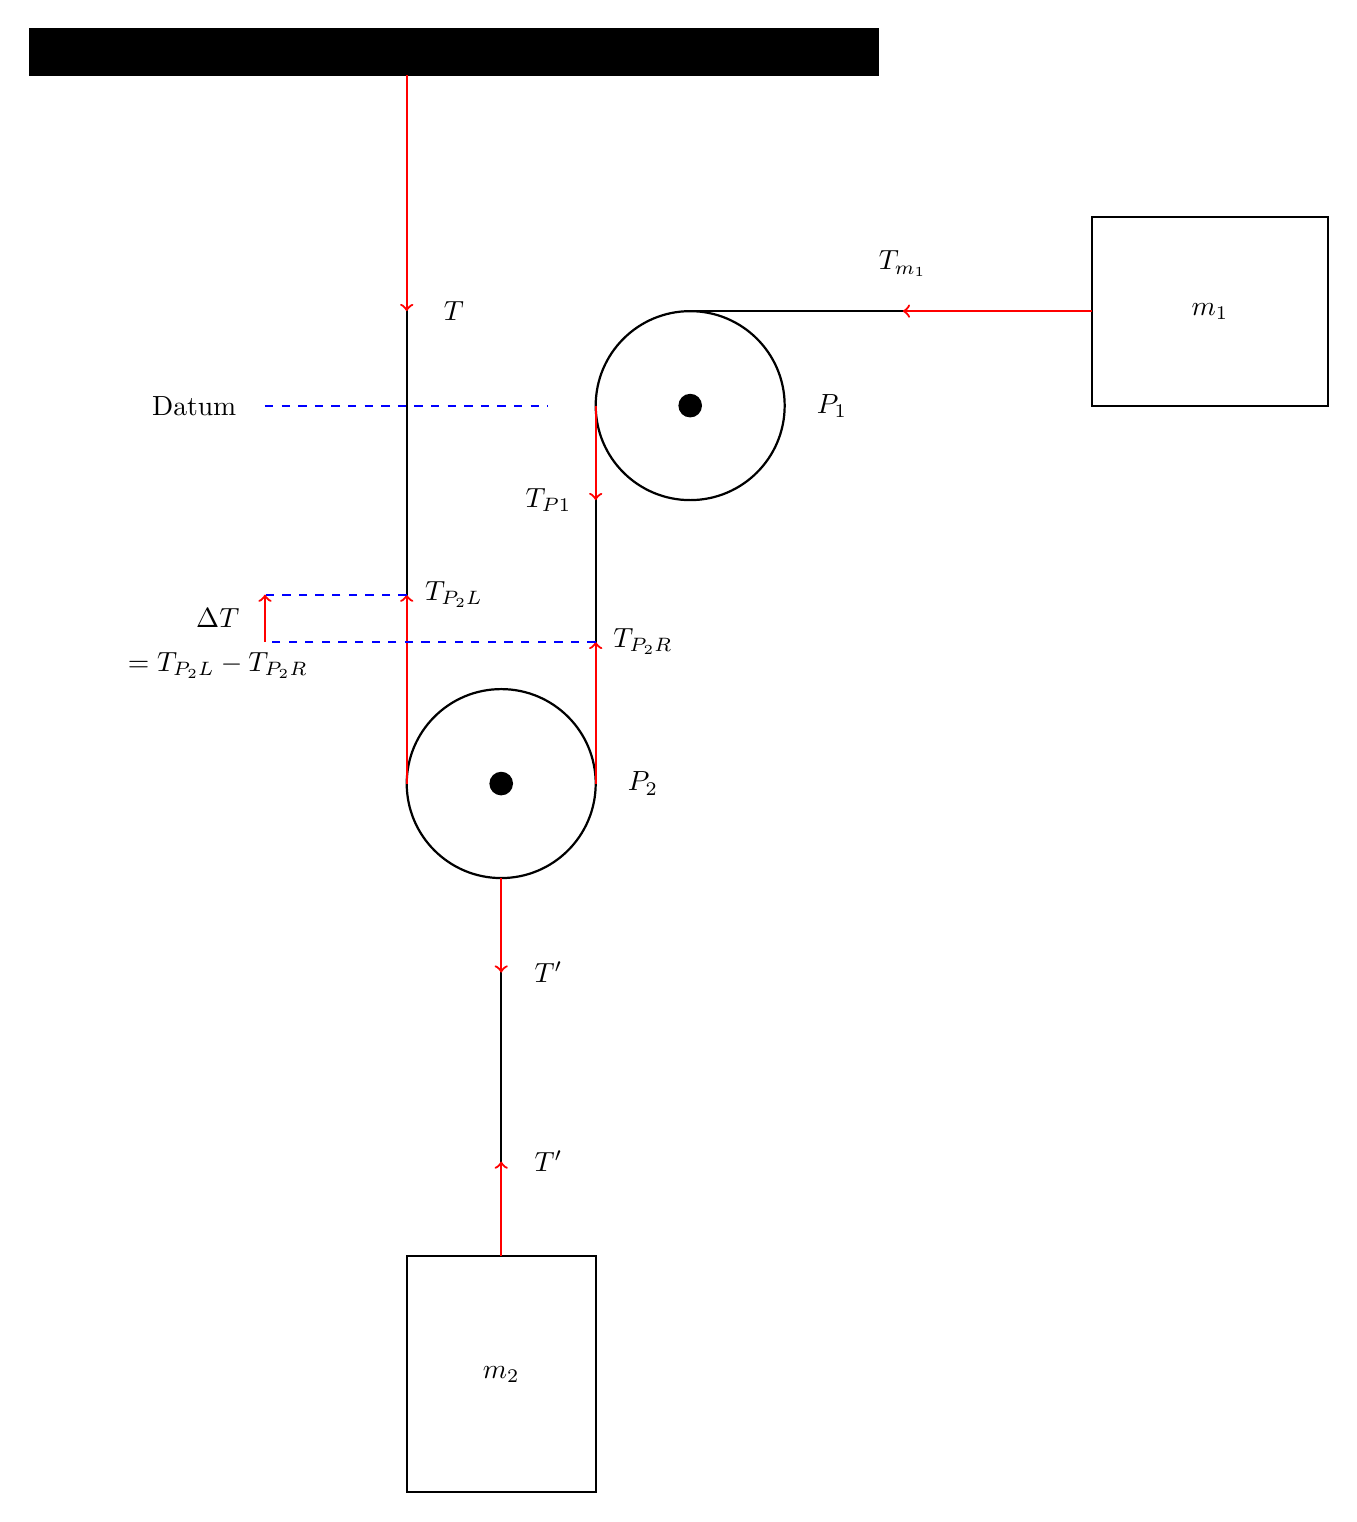
\begin{tikzpicture}[scale=3]

            % Pulley P1
            \draw[thick] (0.8,-1.4) circle (0.4);
            \fill[black] (0.8,-1.4) circle (0.05); % Center of P1
            \node at (0.8+0.6,-1.4) {\(P_1\)}; % Label P1
            
            % Pulley P2
            \draw[thick] (0,-3) circle (0.4);
            \fill[black] (0,-3) circle (0.05); % Center of P2
            \node at (0.6,-3) {\(P_2\)}; % Label P2
            
            % Block m1
            \draw[thick] (2.5,-0.6) -- (2.5,-1.4) -- (3.5,-1.4) -- (3.5,-0.6) -- cycle;
            \node at (3,-1) {\(m_1\)}; % Label m1
            
            % Block m2
            \draw[thick] (-0.4,-5) -- (-0.4,-6) -- (0.4,-6) -- (0.4,-5) -- cycle;
            \node at (0,-5.5) {\(m_2\)}; % Label m2
            
            % Supporting beam
            \draw[thick] (-2,0) -- (1.6,0);
            \fill[black] (-2,0.2) rectangle (1.6,0); % Beam shading
            
            % Strings
            \draw[thick] (2.5,-1) -- (0.8,-1); % String from block m1 to P1
            \draw[thick] (-0.4,0) -- (-0.4,-3); % Support Left to P2
            \draw[thick] (0.4,-1.4) -- (0.4,-3); % Support Left to P2
            \draw[thick] (0,-3.4) -- (0,-5); % String from P2 to block m2

            \draw[thick,->,red] (2.5,-1) -- (1.7,-1); % Tension from block m1 to P1
            \node at (1.7,-1+0.2) {\(T_{m_1}\)}; % Label Tension from block m1 to P1
            \draw[thick,->,red] (-0.4,-3) -- (-0.4,-2.2); % Tension Left to P2
            \node at (-0.4+0.2,-2.2) {\(T_{P_2L}\)}; % Label Tension Left to P2
            \draw[thick,->,red] (0.4,-3) -- (0.4,-2.4); % Tension Right to P2
            \node at (0.4+0.2,-2.4) {\(T_{P_2R}\)}; % Tension Right to P2
            \draw[thick,->,red] (0.4,-1.4) -- (0.4,-1.8); % Tension P1
            \node at (0.4-0.2,-1.8) {\(T_{P1}\)}; % Label Tension P1
            \draw[thick,->,red] (0,-3.4) -- (0,-3.8); % Tension from P2 to block m2
            \node at (0+0.2,-3.8) {\(T'\)}; % Label Tension from P2 to block m2
            \draw[thick,->,red] (0,-5) -- (0,-4.6); % Tension from m2 to block P2
            \node at (0+0.2,-4.6) {\(T'\)}; % Label Tension from m2 to block P2
            \draw[thick,->,red] (-0.4,0) -- (-0.4,-1); % Tension Left to P2
            \node at (-0.4+0.2,-1) {\(T\)}; % Label Tension Left to P2

            \draw[thick,dashed,blue] (-0.4,-2.2) -- (-1,-2.2); % for Delta T
            \draw[thick,dashed,blue] (0.4,-2.4) -- (-1,-2.4); % for Delta T

            \draw[thick,->,red] (-1,-2.4) -- (-1,-2.2); % Tension Left to P2
            \node at (-1-0.2,-2.3) {\(\Delta T\)}; % Label Tension Left to P2
            \node at (-1-0.2,-2.3-0.2) {\(=T_{P_2L}-T_{P_2R}\)}; % Label Tension Left to P2        
            
            \draw[thick,dashed,blue] (-1,-1.4) -- (0.2,-1.4); % Datum

            \node at (-1-0.3,-1.4) {Datum}; % Label Tension Left to P2

        \end{tikzpicture}
    \end{center}

    ai.

    \vspace{12pt}

    This can be intuited by the fact if \(P_2\) drops by \(\delta x\) then to ``fill'' the dropped distance with string it would require \(2\delta x\) of string whilst if \(m_1\) were to move to the left by \(\delta x\) then the ``lost'' string would only be \(\delta x\).
    
    \vspace{12pt}

    Here is the mathematical argument:

    \vspace{12pt}

    Let the total length of the string from a datum be \(l\) then we can express \(l\) as:

    \[l=2x_{p_2}+x_{m_1}+\frac{3}{4}\pi r,\]

    
    where \(x_{p_2}\) is the distance from the datum to \(P_2\)'s left most touch with the string and \(x_{m_1}\) is the distance from the \(P_1\)'s top most touch with the string to \(m_1\) hence by differentiating we get:

    \[0=2v_{p_2}+v_{m_1},\]

    and again:

    \[0=2a_{p_2}+a_{m_1},\]

    where each symbol has its obvious meaning.

    Hence it can be concluded:

    \[2|a_{m_2}|=|a_{m_1}|.\]

    where \(a_{m_2}\) is the acceleration of \(m_2\) as \(m_2\) is a constant displacement from \(P_2\).

    \vspace{12pt}

    ii.

    \vspace{12pt}

    Since \(P_2\) doesn't slip on the left vertical string and is accellerating downwards like \(m_2\) then it must have a rotational acceleration clockwise (the right veritcal string moves so this doesn't apply to the right string), also as \(P_2\) doesn't slip then the tangential acceleration that \(P_2\) falls with at its edge (a distance of \(R\) from its centre) is equal to \(a/2\) where \(a/2\) is it's downwards acceleration and is half \(a\), the magnitude of the acceleration of \(m_1\), by part i. Now for \(P_1\), the string which runs over \(P_1\) is accelearting to the left with an acceleartion \(a\) which is given by the fact that the string is in tension and \(m_1\) is accelearting at \(a\) hence the tangential acceleration at the edge of \(P_1\) is a \(a\) and its rotational acceleration is anticlockwise, thus opposite to the rotational acceleration of \(P_2\). Hence it can be concluded that magnitudes of \(P_1\)'s and \(P_2\)'s rotational acceleration: \(\alpha_{P_1}\), \(\alpha_{P_2}\), respectively, have the relation \(\alpha_{P_1}=2\alpha_{P_2}\) by the fact that their radii are the same and their tangential acceleration are of the same ratio.

    \vspace{12pt}

    b.

    \begin{center}
        \begin{tikzpicture}[scale=1.4]

            % Free-body diagram for m1
            \draw[thick] (-4.5,1) rectangle (-3.5,0);
            \node at (-4, 0.5) {$m_1$};
            \draw[->, thick] (-4, 1) -- (-4, 2.5) node[above] {$R=m_1g$}; % Tension T1
            \draw[->, thick] (-4, 0) -- (-4, -1.5) node[below] {$m_1g$}; % Normal force
            \draw[->, thick] (-3.5, 0.5) -- (-2.5, 0.5) node[right] {$F_f = \mu R = \mu m_1g$}; % Friction force
            \draw[->, thick] (-4.5, 0.5) -- (-6.5, 0.5) node[left] {$T_{m_1}$}; % Tension T2
            \draw[->>, ultra thick] (-1.5,2) -- (-2.5,2) node[left] {$a$};
        
            % Free-body diagram for m2
            \draw[thick] (3.5,1) rectangle (4.5,0);
            \node at (4, 0.5) {$m_2$};
            \draw[->, thick] (4, 1) -- (4, 2) node[above] {$T'$}; % Tension T3
            \draw[->, thick] (4, 0) -- (4, -1.5) node[below] {$m_2 g$}; % Weight of m2
            \draw[->>, ultra thick] (5,2) -- (5,1.5) node[right] {$\frac{a}{2}$};
        
            % Free-body diagram for P1
            \draw[thick] (-4, -4) circle (0.5);
            \node at (-4, -4) {$P_1$};
            \draw[->, thick] (-4, -3) node[right] {$\tau_1=T_{P_1}$} arc (90:220:1); % Torque on P1
            \draw[->>, ultra thick] (-4, -2.5) arc (90:200:1.5) node[below left] {$\alpha=\frac{a}{R}$}; % Torque on P1
            \draw[->, thick] (-4.5, -4) -- (-4.5, -6) node[right] {$T_{P_1}$}; % Tension T P1

        
            % Free-body diagram for P2
            \draw[thick] (4, -5) circle (0.5);n
            \node at (4, -5) {$P_2$};
            \draw[->, thick] (3.5, -5) -- (3.5, -3) node[above] {$T_{P_2L}$}; % Tension T3
            \draw[->, thick] (4.5, -5) -- (4.5, -4.5) node[above left] {$T_{P_2R}$}; % Tension T3
            \draw[->, thick] (3.9, -5.5) -- (3.9, -6.5) node[left] {$T'$}; % Tension from rod
            \draw[->, thick] (4.1, -5.5) -- (4.1, -7.5) node[right] {$Mg$}; % Weight of m2
            \draw[->, thick] (4, -4) arc (90:25:1) node[right] {$\tau_1=T_{P_1}$}; % Torque on P1
            \draw[->>, ultra thick] (4, -3.5) arc (90:35:1.5) node[right] {$\frac{\alpha}{2}=\frac{a}{2R}$}; % Torque on P1

        \end{tikzpicture}
    \end{center}

    c.

    \begin{equation*}
        \begin{tabular}{ |c|c|c|c|c| } 
            \hline
            & \(m_1\) & \(P_1\) & \(m_2\) & \(P_2\) \\
            \hline
            Linear & \(a=\frac{T_{m_1}}{m_1}-\mu g\) & NA & \(2a_{m_2}=a=2g-\frac{2T'}{m_2}\) & \(2a_{P_2}=a=g+\frac{T'-T_{P2L}-T_{P2R}}{M}\) \\
            \hline
            Angular & NA & \(\alpha_{P_1} R=a=\frac{2T_{P_1}}{M}\) & NA & \(\alpha_{P_2} R=\alpha R=a=\frac{4(T_{P2L}-T_{P2R})}{M}\) \\
            \hline
           \end{tabular}
    \end{equation*}

    d.

    \vspace{12pt}

    This is a more useful formulation of what we know:

    \begin{equation*}
        \begin{split}
            T_{m_1}&=am_1+\mu m_1g\\
            T_{P_1}&=\frac{Ma}{2}\\
            T_{P_2L}+T_{P_2R}&=(g-\frac{a}{2})(m_2+M)\qquad\text{this is the linear equation of the \(P_2\) and \(m_2\) system}\\
            T_{P_2L}-T_{P_2R}&=\frac{Ma}{4}\qquad\text{this is the angular equation of the \(P_2\) and \(m_2\) system}\\
        \end{split}
    \end{equation*}

    Now lets look at the tensions in the string

    \begin{center}
        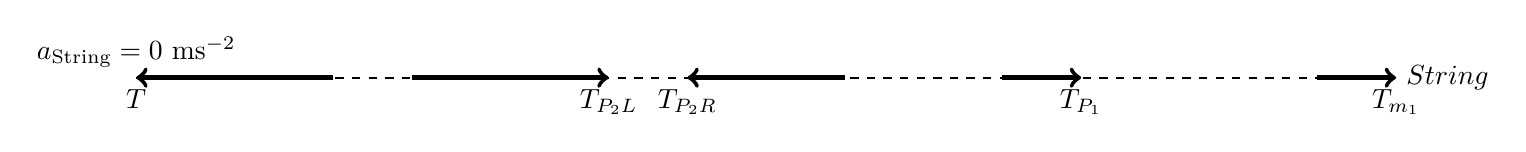
\begin{tikzpicture}
            \draw[thick, dashed] (-8,0)node[above] {$a_{\text{String}}=0\text{ ms\(^{-2}\)}$} -- (8,0) node[right] {$String$}; % String

            \draw[->, ultra thick] (-5.5,0) -- (-8,0) node[below] {$T$}; % T
            \draw[<-, ultra thick] (-2,0)node[below] {$T_{P_2L}$} -- (-4.5,0); % TP2L
            \draw[<-, ultra thick] (-1,0)node[below] {$T_{P_2R}$} -- (1,0); % TP2R
            \draw[->, ultra thick] (3,0) -- (4,0)node[below] {$T_{P_1}$}; % TP1
            \draw[->, ultra thick] (7,0) -- (8,0)node[below] {$T_{m_1}$}; % Tm1

        \end{tikzpicture}
    \end{center}

    (Note: We know that the acceleartion of the string is \(0\) as the string is stationary at the ceiling and as it is inextensible and isn't in compression anywhere it hance cannot accelerate into itself.)

    \vspace{12pt}

    From this illistration it is clear that given the forces are ballenced due to the zero acceleration that:

    \[T+T_{P_2R}=T_{P2L}+T_{P_1}+T_{m_1}\]

    Hence:
    
    \begin{equation}
        \label{noLinearAccelerationEqu}
        T=T_{P2L}-T_{P_2R}+T_{P_1}+T_{m_1}=\frac{3}{4}Ma+m_1a+\mu m_1 g
    \end{equation}

    (Note: This is equation is making use of the angular equation of the \(P_2\) and \(m_1\) system so now our aim is going to be to find a way to make use of the linear equation of the same system.)
    
    \vspace{12pt}
    
    Now to get our final equation note that the implosive and explosive forces on the string must balence everywhere, as the string is inextensible so cannot be streching. Thus if you look at the ends of the string you get the above equation, however if you look at \(P_2\) the implosive forces are: \(T_{P_2L}\), and \(T_{P_2R}\); whilst the explosive forces are: \(T\), \(T_{P_1}\), and \(T_{m_1}\). Hence we are left with the equations. This allows us to make use of our knowledge of \( T_{P_2L}+T_{P_2R}=(g-\frac{a}{2})(m_2+M)\), and allow us to solve for a. Hence:

    \begin{equation}
        \label{implosionExplosionEqu}
        T+T_{P_1}+T_{m_1}=T_{P_2L}+T_{P_2R}=(g-\frac{a}{2})(m_2+M)
    \end{equation}

    And thus by (\ref{noLinearAccelerationEqu}) and (\ref{implosionExplosionEqu}) we get:

    \begin{equation*}
        \frac{3}{4}Ma+m_1a+\mu m_1 g=(g-\frac{a}{2})(m_2+M)
    \end{equation*}

    which once rearranged gives the given answer of:

    \begin{equation*}
        a=\Bigg(\frac{m_2+M-2\mu m_1}{8m_1+2m_2+7M}\Bigg)4g
    \end{equation*}    

\end{document}